\documentclass[12pt]{article}
\usepackage[utf8]{inputenc}
\usepackage[T1]{fontenc}
\usepackage[a4paper, left=2.4cm, right=2.4cm, top=2cm, bottom=2cm, nomarginpar]{geometry}
\usepackage{amsmath, algorithm, pgfplots, pgf, pdfpages, amsfonts, amssymb, stmaryrd, enumitem,graphicx, algpseudocode, setspace, listings, courier, color, caption, centernot, hyperref, lstautogobble, zi4, mathtools, lmodern, colortbl, array, multicol, fancyhdr, lastpage, svg}
\usepackage{booktabs}
\hypersetup{
    pdftitle={CE204_FP1_G6},
    pdftoolbar=true,        % show Acrobat’s toolbar?
    pdfmenubar=true,        % show Acrobat’s menu?
    pdfauthor={Muhammet Yağcıoğlu},
    pdfsubject={CE204_FP_RPs},
    pdfcreator={Muhammet Yağcıoğlu},   % creator of the document
    pdfproducer={Muhammet Yağcıoğlu}, % producer of the document
    colorlinks,
    linkcolor={black},
    citecolor={black},
    urlcolor={blue!80!black}
}
\usepackage[noblocks]{authblk}
\usepackage[version=4]{mhchem}
\usepackage[export]{adjustbox}
\usepackage{eso-pic} % Required for absolute positioning
\graphicspath{ {./images/} }
\usetikzlibrary{patterns}
\usepackage{tikz-3dplot}
\usepackage[version=4]{mhchem}
\usepackage[export]{adjustbox}
\usepgfplotslibrary{groupplots}
\usepackage{xcolor}
\usepackage[absolute,overlay]{textpos}
\usepackage{ragged2e}
\usepackage{xcolor}
\usepackage{amsthm}
\usepackage{tikz}




%----------compiler settings---------
\setlength{\parindent}{0pt}
\everymath{\displaystyle}
\onehalfspacing

%-----------colors----------
\pgfplotsset{compat=1.18}
\definecolor{bluekeywords}{rgb}{0.13, 0.13, 1}
\definecolor{greencomments}{rgb}{0, 0.5, 0}
\definecolor{redstrings}{rgb}{0.9, 0, 0}
\definecolor{graynumbers}{rgb}{0.5, 0.5, 0.5}
\definecolor{bronze}{rgb}{0.82, 0.41, 0.12}
\definecolor{crimson}{rgb}{0.86, 0.08, 0.24}
\definecolor{brown(web)}{rgb}{0.65, 0.16, 0.16}
\definecolor{darkspringgreen}{rgb}{0.16, 0.32, 0.75}
\definecolor{blue(ncs)}{rgb}{0.0, 0.53, 0.74}
\definecolor{amber}{rgb}{1.0, 0.49, 0.0}
\definecolor{cadmiumgreen}{rgb}{0.0, 0.42, 0.24}




%-------code frame-----------
\lstset{
    autogobble,
    columns=fullflexible,
    showspaces=false,
    showtabs=false,
    breaklines=true,
    showstringspaces=false,
    breakatwhitespace=true,
    escapeinside={(*@}{@*)},
    commentstyle=\color{greencomments},
    keywordstyle=\color{bluekeywords},
    stringstyle=\color{redstrings},
    numberstyle=\color{graynumbers},
    basicstyle=\ttfamily\footnotesize,
    frame=l,
    framesep=12pt,
    xleftmargin=12pt,
    tabsize=4,
    captionpos=b
}



\lstdefinelanguage{myMMA}{
keywords={SetDirectory, NotebookDirectory, Exp, IdentityMatrix, Eigenvalues, 
ListPlot, PlotRange, PlotStyle, Directive, PointSize, AspectRatio, Blue, Graphics, Line, 
Manipulate, Show, Sqrt, UniformDistribution, GammaDistribution, BetaDistribution, 
Nintegrate, For, DataRange, AxesLabel, PlotLabel, Transpose, Export, Plot, Append, Infinity},
keywordstyle=\color{black},
commentstyle=\color{gray}, 
identifierstyle=\color{blue},
sensitive=false,
comment=[l]{(*},
morecomment=[s]{/*}{*/},
morestring=[b]',
morestring=[b]"
}






%-----gauss declare---------
\pgfmathdeclarefunction{gauss}{2}{%
  \pgfmathparse{1/(#2*sqrt(2*pi)) * exp(-((x-#1)^2)/(2*#2^2))}%
}
\usetikzlibrary{arrows.meta, decorations.markings}
\pgfplotsset{compat=1.17}







%--------------page numbering------------
\fancyfoot[R]{page \thepage\ of \textcolor{bronze}{\pageref{LastPage}}}
\fancyhead[R]{Group 6}



%-------------qframe settings---------------

\usepackage[framemethod=TikZ]{mdframed}
\newmdenv[%
    skipabove=1em, % space above the frame
    skipbelow=1em, % space below the frame
    linewidth=1pt, % width of the frame lines
    linecolor=gray!80, % color of the frame lines
    backgroundcolor=gray!9, % background color inside the frame
    roundcorner=5pt, % radius of the rounded corners
    innerleftmargin=1em, % margin within the frame at the left
    innerrightmargin=1em, % margin within the frame at the right
    innertopmargin=0.5em, % margin within the frame at the top
    innerbottommargin=0.5em % margin within the frame at the bottom
]{qframe}

\newenvironment{q}
{
    \begin{qframe}
    \noindent\textit{\textbf{Problem Statement:}}
    \par\smallskip
}
{
    \end{qframe}
}





%-------------ANSWER TAG---------------
\newcommand{\AnswerTag}{\hfill 
\begin{tikzpicture} \fill[black] (0.35cm,0) -- (0,0.175cm) -- (0.35cm,0.35cm) -- cycle;\end{tikzpicture}}



%-------Theorem and another question frames----------
\newenvironment{theorem}{\begin{mdframed}\textbf{Theorem.}}{\end{mdframed}}

%usage: \begin{theorem}

\newenvironment{question}{\begin{mdframed}\textbf{Question.}}{\end{mdframed}}

%usage: %usage: \begin{question}
\usepackage{hyperref} 
\hypersetup{
    pdftoolbar=true,        % show Acrobat’s toolbar?
    pdfmenubar=true,        % show Acrobat’s menu?
    pdffitwindow=false,     % window fit to page when opened
    pdfstartview={FitH},    % fits the width of the page to the window
    pdftitle={MuhammetYagcioglu - CE231 HW2},    % title
    pdfauthor={Muhammet Yağcıoğlu},     % author
    pdfsubject={CE231 HW2},   % subject of the document
    pdfcreator={Muhammet Yağcıoğlu},   % creator of the document
    pdfproducer={Muhammet Yağcıoğlu}, % producer of the document
    pdfnewwindow=true,      % links in new window
    colorlinks=true,       % false: boxed links; true: colored links
    linkcolor=red,          % color of internal links (change box color with linkbordercolor)
    citecolor=green,        % color of links to bibliography
    filecolor=magenta,      % color of file links
    urlcolor=cyan,           % color of external links
    pdfpagemode=FullScreen
}
\usepackage{sectsty}
\title{\vspace{-1cm}CE231 - Engineering Economy HW2}
\author{Muhammet Yağcıoğlu - 290204042}

\fancyhead[L]{\textbf{CE 231, Engineering Economy, Fall 2023, HW2}}


\begin{document}
\pagestyle{fancy}
\maketitle\thispagestyle{fancy}

\tableofcontents

\newpage
\section*{Question 1}
\addcontentsline{toc}{section}{Question 1}
\begin{q}
1. (30 pts.) Three mutually exclusive design alternatives are being considered. The estimated cash flows for each alternative are given in the table below. The MARR of the company is \(20 \%\) per year. At the end of its useful life, the investment will be sold with end-of-life market values given in the table.

\begin{center}
\begin{tabular}{llll} 
& A & B & C \\
\cline { 2 - 4 } Investment cost & \(\$ 28,000\) & \(\$ 55,000\) & \(\$ 40,000\) \\
Annual expenses & \(\$ 15,000\) & \(\$ 13,000\) & \(\$ 22,000\) \\
Annual revenues & \(\$ 23,000\) & \(\$ 28,000\) & \(\$ 32,000\) \\
Market value at the end of life & \(\$ 6,000\) & \(\$ 8,000\) & \(\$ 10,000\) \\
Useful life & 10 years & 10 years & 10 years \\
IRR & \(26.4 \%\) & \(24.7 \%\) & \(22.4 \%\)
\end{tabular}
\end{center}

(a) Explain why the decision should not be made by comparing IRR values for the three alternatives.

(b) Recommend the best alternative by using an appropriate method.
\end{q}

\begin{figure}[!ht]
\centering
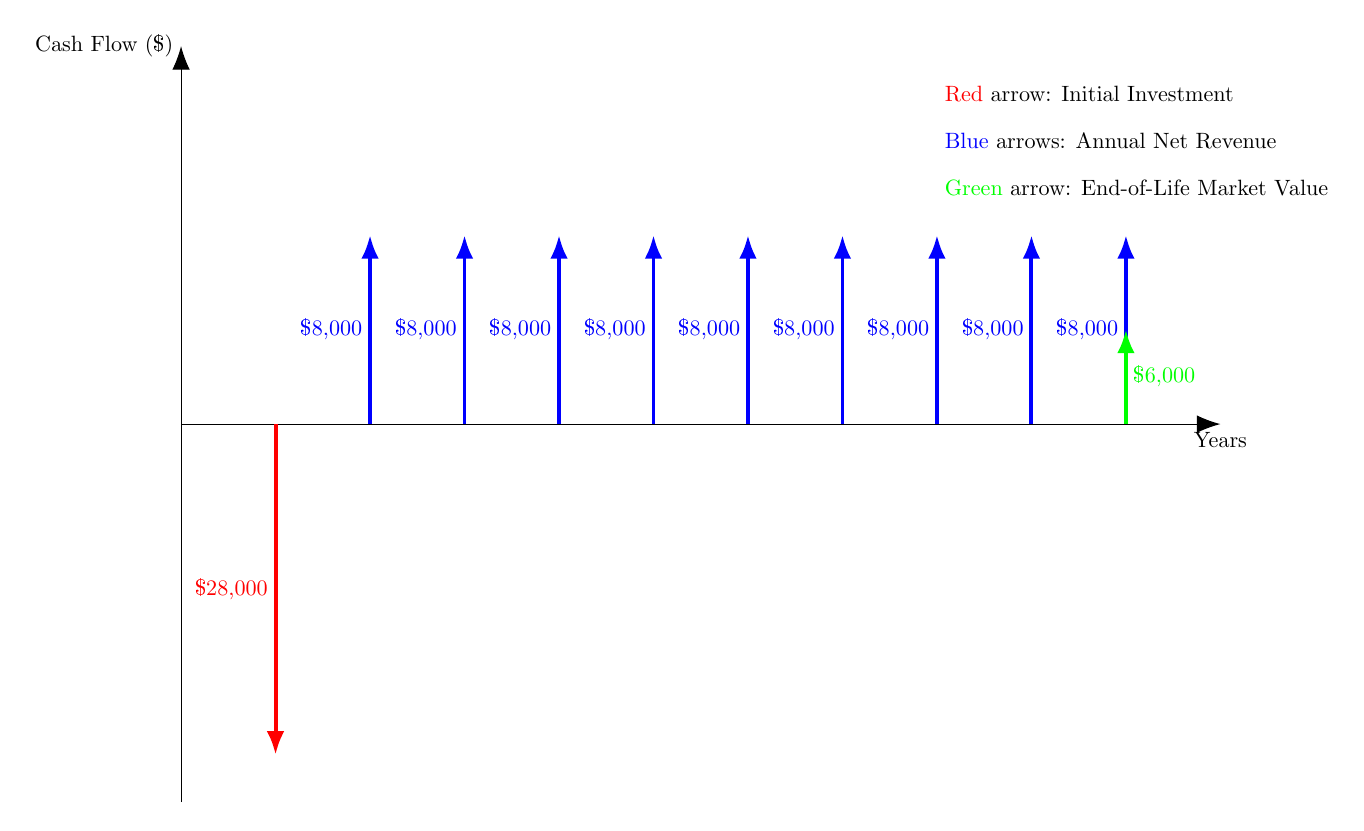
\begin{tikzpicture}[scale=1.2, every node/.style={scale=0.8}]
    % Draw axes
    \draw[-{Latex[length=3mm]}] (0,0) -- (11,0) node[anchor=north] {Years};
    \draw[-{Latex[length=3mm]}] (0,-4) -- (0,4) node[anchor=east] {Cash Flow (\$)};

    % Initial investment for A
    \draw[red, line width=0.5mm, -{Latex[length=3mm]}] (1,0) -- (1,-3.5);
    \node[red, anchor=east] at (1, -1.75) {\$28,000};

    % Annual net revenue (Revenue - Expense)
    \foreach \y in {2,3,...,10} {
        \draw[blue, line width=0.5mm, -{Latex[length=3mm]}] (\y,0) -- (\y,2);
        \node[blue, anchor=east] at (\y, 1) {\$8,000};
    }

    % Market value at the end of life
    \draw[green, line width=0.5mm, -{Latex[length=3mm]}] (10,0) -- (10,1);
    \node[green, anchor=west] at (10, 0.5) {\$6,000};

    % Adding labels
    \node[align=left, anchor=west] at (8, 3.5) {\textcolor{red}{Red} arrow: Initial Investment};
    \node[align=left, anchor=west] at (8, 3) {\textcolor{blue}{Blue} arrows: Annual Net Revenue};
    \node[align=left, anchor=west] at (8, 2.5) {\textcolor{green}{Green} arrow: End-of-Life Market Value};

\end{tikzpicture}
\caption{Cash Flow Diagram for Alternative A}
\end{figure}


\begin{figure}[!ht]
\centering
\begin{tikzpicture}[scale=1, every node/.style={scale=0.6}]
    % Draw axes
    \draw[-{Latex[length=3mm]}] (0,0) -- (11,0) node[anchor=north] {Years};
    \draw[-{Latex[length=3mm]}] (0,-6) -- (0,6) node[anchor=east] {Cash Flow (\$)};

    % Initial investment for B
    \draw[red, line width=0.5mm, -{Latex[length=3mm]}] (1,0) -- (1,-5.5);
    \node[red, anchor=east] at (1, -2.75) {\$55,000};

    % Annual net revenue (Revenue - Expense)
    \foreach \y in {2,3,...,10} {
        \draw[blue, line width=0.5mm, -{Latex[length=3mm]}] (\y,0) -- (\y,3);
        \node[blue, anchor=east] at (\y, 1.5) {\$15,000};
    }

    % Market value at the end of life
    \draw[green, line width=0.5mm, -{Latex[length=3mm]}] (10,0) -- (10,1.6);
    \node[green, anchor=west] at (10, 0.8) {\$8,000};
\end{tikzpicture}
\caption{Cash Flow Diagram for Alternative B}
\end{figure}

\begin{figure}[!ht]
\centering
\begin{tikzpicture}[scale=1, every node/.style={scale=0.6}]
    % Draw axes
    \draw[-{Latex[length=3mm]}] (0,0) -- (11,0) node[anchor=north] {Years};
    \draw[-{Latex[length=3mm]}] (0,-5) -- (0,5) node[anchor=east] {Cash Flow (\$)};

    % Initial investment for C
    \draw[red, line width=0.5mm, -{Latex[length=3mm]}] (1,0) -- (1,-4);
    \node[red, anchor=east] at (1, -2) {\$40,000};

    % Annual net revenue (Revenue - Expense)
    \foreach \y in {2,3,...,10} {
        \draw[blue, line width=0.5mm, -{Latex[length=3mm]}] (\y,0) -- (\y,2);
        \node[blue, anchor=east] at (\y, 1) {\$10,000};
    }

    % Market value at the end of life
    \draw[green, line width=0.5mm, -{Latex[length=3mm]}] (10,0) -- (10,2);
    \node[green, anchor=west] at (10, 1) {\$10,000};
\end{tikzpicture}
\caption{Cash Flow Diagram for Alternative C}
\end{figure}


\newpage
\subsection*{Part a}
\addcontentsline{toc}{subsection}{Part a}
Consider the set \(\mathcal{A} = \{A, B, C\}\) representing the three investment alternatives. Each element \( \alpha \in \mathcal{A} \) is associated with a tuple \((I_\alpha, R_\alpha, E_\alpha, M_\alpha, n, \text{IRR}_\alpha)\), where \( I_\alpha \) denotes the initial investment cost,\( R_\alpha \) denotes the annual revenue,\( E_\alpha \) denotes the annual expense,\( M_\alpha \) denotes the market value at the end of life, \( n \) denotes the useful life span (assumed constant across \(\mathcal{A}\)), \( \text{IRR}_\alpha \) denotes the Internal Rate of Return. Given the Minimum Acceptable Rate of Return (MARR), denoted as \( i \), the task is to ascertain the most viable alternative based on economic metrics. In part (a), the fallacy of relying solely on IRR values for decision making is to be demonstrated. For this purpose, consider the function \( \mathcal{F}: \mathcal{A} \to \mathbb{R} \), defined as \(\mathcal{F}(\alpha) = \text{IRR}_\alpha\). The argument posits that while \(\mathcal{F}\) provides a rate of return relative to the initial investment, it does not encapsulate the absolute monetary return nor the scale of investment. To illustrate this, let \( \mathcal{P} \) be a set of two hypothetical projects, with \(\mathcal{P} = \{P_1, P_2\}\), where each \(P_j\) is defined by \((I_j, r_j)\), representing investment and rate of return respectively. Suppose \(I_1 \gg I_2\) and \(r_1 < r_2\) but \(\frac{I_1 \cdot r_1}{1} > \frac{I_2 \cdot r_2}{1}\). This denotes a scenario where a larger investment with a lower rate of return yields a higher absolute return than a smaller investment with a higher rate of return, thereby challenging the notion of IRR supremacy. So, in other words, let \(\mathcal{G}: \mathcal{P} \to \mathbb{R}\) be defined as \(\mathcal{G}(P_j) = I_j \cdot r_j\). The proposition is that \(\exists P_1, P_2 \in \mathcal{P}\) such that \(I_1 \cdot r_1 > I_2 \cdot r_2\) despite \(r_1 < r_2\). In conclusion, the decision criterion must extend beyond the scope of the IRR and incorporate other financial metrics that offer a more holistic view of the economic implications of each investment alternative. This necessitates a transition to methodologies like Present Worth (PW) and Annual Worth (AW) analysis for a more comprehensive evaluation, as will be expounded in part (b) of the solution.
\subsection*{Part b}
\addcontentsline{toc}{subsection}{Part b}

Let us define a manifold \(\mathcal{M}\) representing the financial state-space of the problem. Each point in \(\mathcal{M}\) corresponds to a unique financial scenario characterized by a set of parameters like investment cost, revenue, expenses, and market values over time. The trajectories in \(\mathcal{M}\) are not defined by differential equations, but by algebraic financial formulas that map the financial state at one point in time to another. For each alternative \(\alpha \in \mathcal{A}\), we compute the Present Worth (PW) and Annual Worth (AW) as follows:

\textit{Present Worth (PW) Calculation}

Let \(\text{PW}(\alpha)\) be the present worth of alternative \(\alpha\). It is given by: \[ \text{PW}(\alpha) = -I_\alpha + (R_\alpha - E_\alpha) \cdot (P/A, i, n) + M_\alpha \cdot (P/F, i, n). \] The terms \((P/A, i, n)\) and \((P/F, i, n)\) are the present worth factors. For the given data: - \(I_A = \$28,000\), \(R_A - E_A = \$8,000\), \(M_A = \$6,000\) - \(I_B = \$55,000\), \(R_B - E_B = \$15,000\), \(M_B = \$8,000\) - \(I_C = \$40,000\), \(R_C - E_C = \$10,000\), \(M_C = \$10,000\). Substituting these into the \(\text{PW}\) formula yields \[P W_A=-\$ 28,000+(\$ 23,000-\$ 15,000)(P / A, 20 \%, 10)+\$ 6,000(P / F, 20 \%, 10)=\$ 6,509\] \[P W_B=-\$ 55,000+(\$ 28,000-\$ 13,000)(P / A, 20 \%, 10)+\$ 8,000(P / F, 20 \%, 10)=\$ 9,180\] \[P W_C=-\$ 40,000+(\$ 32,000-\$ 22,000)(P / A, 20 \%, 10)+\$ 10,000(P / F, 20 \%, 10)=\$ 3,540\]

\textit{Annual Worth (AW) Calculation}

The Annual Worth \(\text{AW}(\alpha)\) for each alternative is computed using the relationship: \[ \text{AW}(\alpha) = \text{PW}(\alpha) \cdot (A/P, i, n) \] where \((A/P, i, n)\) is the capital recovery factor. This yields \[\begin{aligned} & A W_A=\$ 6,509(A / P, 20 \%, 10)=6509(0.2385)=\$ 1552.4 \\ & \boxed{A W_B=\$ 9,180(A / P, 20 \%, 10)=9180(0.2385)=\$ 2189.4} \\ & A W_C=\$ 3,540(A / P, 20 \%, 10)=3540(0.2385)=\$ 844.29 \end{aligned}\]
   

The alternative \(\alpha^*\) that maximizes \(\text{PW}(\alpha)\) (and consequently \(\text{AW}(\alpha)\)) is identified as the most financially advantageous choice. The maximization problem is stated as:
\[ \alpha^* = \underset{\alpha \in \mathcal{A}}{\arg\max} \, \text{PW}(\alpha) \]

Thus, the \underline{Alternative B is the best alternative} among the three.


\newpage
\section*{Question 2}
\addcontentsline{toc}{section}{Question 2}
\begin{q}
2. (30 pts.) A company is considering replacing a machine (defender) that was bought six years ago for \(\$ 50,000\) and has now malfunctioned. The machine can be repaired to extend its life by five more years. If repaired, the machine will require an operating cost of \(\$ 10,000\) per year. If it is replaced, the new machine (challenger) will cost \(\$ 44,000\), will last for six years, and will have operating expenses of \(\$ 5,000\) per year. The challenger will have zero salvage value at the end of its six year life. The malfunctioned defender can be sold at a current market value of \(\$ 15,000\). If MARR is \(12 \%\) per year, what is the maximum amount that the company should spend to repair the existing machine instead of switching to the challenger? Use the outsider viewpoint method. (Note: All values are before taxes, no tax calculations are necessary).
\end{q}



\begin{figure}[!ht]
    \centering
    \begin{tikzpicture}[scale=1.5, every node/.style={scale=0.8}]
        % Draw axes
        \draw[-{Latex[length=3mm]}] (0,0) -- (6,0) node[anchor=north] {Years};
        \draw[-{Latex[length=3mm]}] (0,0) -- (0,4) node[anchor=east] {Cash Flow (\$)};

        % Time markers
        \foreach \x in {0,1,...,5} {
            \draw (\x,3pt) -- (\x,-3pt) node[anchor=north] {\x};
        }

        % Defender cash flows
        % Repair cost (Year 0)
        \draw[red, line width=0.5mm, -{Latex[length=3mm]}] (0,0) -- (0,-2) node[anchor=east] {$X$};
        % Operating costs (Years 1 to 5)
        \foreach \x in {1,2,...,5} {
            \draw[red, line width=0.5mm, -{Latex[length=3mm]}] (\x,0) -- (\x,-1) node[midway, left] {\$10,000};
        }
        % Salvage value (Year 5)
        \draw[red, line width=0.5mm, -{Latex[length=3mm]}] (5,0) -- (5,1.5) node[anchor=west] {\$15,000};

        % Challenger cash flows
        % Initial cost (Year 0)
        \draw[blue, line width=0.5mm, -{Latex[length=3mm]}] (0.5,0) -- (0.5,-3) node[anchor=east] {\$44,000};
        % Operating costs (Years 1 to 5)
        \foreach \x in {1.5,2.5,...,5.5} {
            \draw[blue, line width=0.5mm, -{Latex[length=3mm]}] (\x,0) -- (\x,-0.5) node[midway, right] {\$5,000};
        }
    \end{tikzpicture}
    \caption{Cash Flow Diagram for Defender vs. Challenger}
    \label{fig:defender-vs-challenger}
\end{figure}
Let us define \(X\) as the variable representing the repair cost of the Defender, a real number within the domain \(\mathbb{R}\). The goal is to ascertain the upper bound of \(X\) for which the repair of the Defender remains economically justified in contrast to the procurement of the Challenger. We proceed by evaluating the Annual Worth (AW) of both the Defender and Challenger. The AW is a financial metric that translates various costs and benefits occurring at different times into a uniform series of annual values, thereby facilitating a direct comparison. For the Defender (denoted as \(D\)) and Challenger (denoted as \(C\)), we define their respective AW functions, \(AW_D\) and \(AW_C\), as follows: \begin{align*} AW_D = -O_D - (S_D + X) \times \text{CRF}(i, n_D) \\ AW_C = -O_C - C_C \times \text{CRF}(i, n_C) \end{align*} Here, \(O_D\) and \(O_C\) represent the annual operating costs of \(D\) and \(C\), respectively. \(S_D\) is the salvage value of \(D\), \(C_C\) is the cost of \(C\), \(n_D\) and \(n_C\) are their respective operational lifespans, and \(i\) is the MARR. The term \(\text{CRF}(i, n)\) denotes the capital recovery factor, a function encapsulating the conversion of a present value into an equivalent annual value over \(n\) periods at an interest rate \(i\). Upon substitution of the given monetary values and applying the respective CRF values, the inequalities representing the economic comparison between \(D\) and \(C\) are formulated. The decision criterion hinges on the condition \(AW_D \geq AW_C\), which, when applied, results in an inequality to solve for \(X\): \[ -10,000 - (15,000 + X) \times 0.2774 \geq -5,000 - 44,000 \times 0.2432 .\] The solution to this inequality will yield the maximum permissible value for \(X\). \[\boxed{X \leq \$ 5550.83}.\] So, as long as the repair cost is less than \(\$ \textit{5550.83}\), \textbf{D} should be kept in service, otherwise replaced.

\newpage
\section*{Question 3}
\addcontentsline{toc}{section}{Question 3}
\begin{q}
3. (40 pts.) Anew forklift truck will require an investment of \(\$ 30,000\) and is expected to have end-of-year market values and annual expenses as shown in the Table below. If MARR is \(10 \%\) per year, find the Economic Service Life of the truck.
\begin{center}
\begin{tabular}{lll} 
End of year & \begin{tabular}{l} 
Market Value \\
at end of year
\end{tabular} & \begin{tabular}{l} 
Annual Expenses \\
during year
\end{tabular} \\
\hline \hline 1 & \(\$ 22,500\) & \(\$ 3,000\) \\
2 & \(\$ 16,875\) & \(\$ 4,500\) \\
3 & \(\$ 12,750\) & \(\$ 7,000\) \\
4 & \(\$ 9,750\) & \(\$ 10,000\) \\
5 & \(\$ 7,125\) & \(\$ 13,000\)
\end{tabular}
\end{center}
\end{q}

\begin{figure}[!ht]
    \centering
    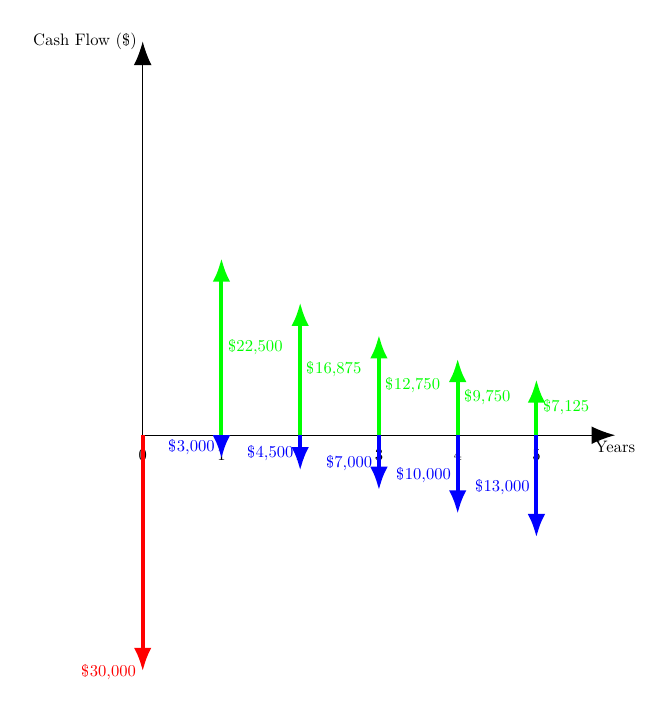
\begin{tikzpicture}[scale=1, every node/.style={scale=0.6}]
        % Draw axes
        \draw[-{Latex[length=3mm]}] (0,0) -- (6,0) node[anchor=north] {Years};
        \draw[-{Latex[length=3mm]}] (0,0) -- (0,5) node[anchor=east] {Cash Flow (\$)};

        % Time markers
        \foreach \x in {0,1,...,5} {
            \draw (\x,3pt) -- (\x,-3pt) node[anchor=north] {\x};
        }
        % Initial investment at Year 0 (30,000)
        \draw[red, line width=0.5mm, -{Latex[length=3mm]}] (0,0) -- (0,-3) node[anchor=east] {\$30,000};
    
        % Annual expenses and market values for each year
        % Year 1 (Expense: 3,000, Market Value: 22,500)
        \draw[blue, line width=0.5mm, -{Latex[length=3mm]}] (1,0) -- (1,-0.3) node[midway, left] {\$3,000};
        \draw[green, line width=0.5mm, -{Latex[length=3mm]}] (1,0) -- (1,2.25) node[midway, right] {\$22,500};
    
        % Year 2 (Expense: 4,500, Market Value: 16,875)
        \draw[blue, line width=0.5mm, -{Latex[length=3mm]}] (2,0) -- (2,-0.45) node[midway, left] {\$4,500};
        \draw[green, line width=0.5mm, -{Latex[length=3mm]}] (2,0) -- (2,1.6875) node[midway, right] {\$16,875};
    
        % Year 3 (Expense: 7,000, Market Value: 12,750)
        \draw[blue, line width=0.5mm, -{Latex[length=3mm]}] (3,0) -- (3,-0.7) node[midway, left] {\$7,000};
        \draw[green, line width=0.5mm, -{Latex[length=3mm]}] (3,0) -- (3,1.275) node[midway, right] {\$12,750};
    
        % Year 4 (Expense: 10,000, Market Value: 9,750)
        \draw[blue, line width=0.5mm, -{Latex[length=3mm]}] (4,0) -- (4,-1) node[midway, left] {\$10,000};
        \draw[green, line width=0.5mm, -{Latex[length=3mm]}] (4,0) -- (4,0.975) node[midway, right] {\$9,750};
    
        % Year 5 (Expense: 13,000, Market Value: 7,125)
        \draw[blue, line width=0.5mm, -{Latex[length=3mm]}] (5,0) -- (5,-1.3) node[midway, left] {\$13,000};
        \draw[green, line width=0.5mm, -{Latex[length=3mm]}] (5,0) -- (5,0.7125) node[midway, right] {\$7,125};

\end{tikzpicture}
\caption{Cash Flow Diagram for Forklift Truck Investment}
\label{fig:forklift-truck-investment}
\end{figure}

Let \( I = \$30,000 \) be the initial investment, \( r = 10\% \) be the MARR, \( V(t) \) be the market value at the end of year \( t \), and \( E(t) \) be the annual expenses during year \( t \). The values of \( V(t) \) and \( E(t) \) for \( t = 1, 2, 3, 4, 5 \) are provided in the problem statement. The EUAC for a given year \( t \) is the sum of the annualized initial investment and the annualized sum of expenses and salvage values, which can be calculated using the formula for the present worth of an annuity. The EUAC for year \( t \) is given by: \[ \text{EUAC}(t) = \frac{I - V(t)(P/F, r, t)}{(P/A, r, t)} + \sum_{i=1}^{t} E(i)(P/F, r, i)(A/P, r, t) \] To minimize EUAC, we compute the EUAC for each year \( t \) from 1 to 5 and identify the year \( t^* \) for which EUAC is minimum. This year represents the optimal economic service life of the truck. \begin{center} \begin{tabular}{rrrrrr} \toprule Year (t) & Market Value (V(t)) & P/F & P/A & Cumulative Expenses & EUAC \\ \midrule 1 & 22500 & 0.91 & 1.10 & 2727.27 & 13500.00 \\ 2 & 16875 & 0.83 & 0.58 & 6446.28 & 12964.29 \\ 3 & 12750 & 0.75 & 0.40 & 11705.48 & 12918.43 \\ 4 & 9750 & 0.68 & 0.32 & 18535.62 & 13210.73 \\ 5 & 7125 & 0.62 & 0.26 & 26607.60 & 13765.88 \\ \bottomrule \end{tabular} \end{center} These calculations are executed for each year, and the results are compared to determine the minimum EUAC. The year corresponding to this minimum value is the solution \( t^* \), which represents the economic service life of the truck. The task is to find \( t^* \) such that \[ t^* = \underset{t \in \{1, 2, 3, 4, 5\}}{\mathrm{argmin}} \, \text{EUAC}(t). \] Given the EUAC values: 

\begin{table}[h] \centering \begin{tabular}{|c|c|} \hline \textbf{Year} (\(t\)) & \textbf{EUAC} \\ \hline 1 & \$13,500.00 \\ 2 & \$12,964.29 \\ 3 & \$12,918.43 \\ 4 & \$13,210.73 \\ 5 & \$13,765.88 \\ \hline \end{tabular} \caption{Equivalent Uniform Annual Costs (EUAC) for Each Year} \label{tab:euac_values} \end{table} We observe that the EUAC is minimized for \( t = 3 \). Therefore, it follows that \[ \boxed{t^* = 3}. \] This implies that the optimal economic service life of the forklift truck is \textit{3} years.

\newpage
\subsection*{MATLAB/Python Algorithm Table}
\addcontentsline{toc}{subsection}{MATLAB/Python Algorithm Table}
\begin{algorithm}
\caption{Calculate Economic Service Life of a Forklift Truck}
\begin{algorithmic}[1]

\State $I \gets 30000$ \Comment{Initial investment}
\State $r \gets 0.10$ \Comment{Minimum Attractive Rate of Return (MARR)}
\State Define $years \gets \{1, 2, 3, 4, 5\}$
\State Define $market\_values \gets \{22500, 16875, 12750, 9750, 7125\}$
\State Define $annual\_expenses \gets \{3000, 4500, 7000, 10000, 13000\}$
\State Initialize an empty list $euac\_values$

\Function{PresentWorthFactor}{$r, t$}
    \State \Return $\frac{1}{(1 + r)^t}$
\EndFunction

\Function{CapitalRecoveryFactor}{$r, t$}
    \State \Return $\frac{r}{1 - (1 + r)^{-t}}$
\EndFunction

\Function{SeriesPresentWorthFactor}{$r, t$}
    \State \Return $\frac{r(1 + r)^t}{(1 + r)^t - 1}$
\EndFunction

\For{$year \in years$}
    \State $p\_f \gets \Call{PresentWorthFactor}{r, year}$
    \State $p\_a \gets \Call{CapitalRecoveryFactor}{r, year}$
    \State $cumulative\_expense \gets \sum_{i=1}^{year} annual\_expenses[i] \times \Call{PresentWorthFactor}{r, i}$
    \State $euac \gets (I - market\_values[year - 1] \times p\_f) \times p\_a + cumulative\_expense \times \Call{SeriesPresentWorthFactor}{r, year}$
    \State Add $euac$ to $euac\_values$
\EndFor

\State Prepare and display the results in a structured format

\end{algorithmic}
\end{algorithm}

\end{document}
